\documentclass{beamer}

\mode<presentation> {


\usetheme{default}
% \setbeamertemplate{footline} % To remove the footer line in all slides uncomment this line
\setbeamertemplate{footline}[page number] % To replace the footer line in all slides with a simple slide count uncomment this line
\setbeamertemplate{navigation symbols}{} % To remove the navigation symbols from the bottom of all slides uncomment this line
}

\usepackage{graphicx} % Allows including images
\usepackage{booktabs} % Allows the use of \toprule, \midrule and \bottomrule in tables
\usepackage{verbatim}
\usepackage{multicol}

\title[VE215 RC2]{VE215 RC2}
\author{Erdao Liang, Chongye Yang}
\institute[UM-SJTU JI] 
{UM-SJTU JI}
\date{\today}

\begin{document}

\AtBeginSection[ ]
{
\begin{frame}{Overview}
    \tableofcontents[sectionstyle=show/shaded,subsectionstyle=show/shaded/hide]
 \end{frame}
}

%%%%%%%%%%%%%%%%%%%%%%%%%%%%%%%%%%%%%%%%%%%%%%%%%%%
% TITLE PAGE
\begin{frame}
\titlepage % Print the title page as the first slide
\end{frame}

%%%%%%%%%%%%%%%%%%%%%%%%%%%%%%%%%%%%%%%%%%%%%%%%%%%
% OVERVIEW
% \begin{frame}
% \frametitle{Overview}
% \tableofcontents
% \end{frame}

%%%%%%%%%%%%%%%%%%%%%%%%%%%%%%%%%%%%%%%%%%%%%%%%%%%
% CIRCUIT THEOREMS
\section{Circuit Theorems}

\begin{frame}{Overview-Chapter4 Circuit Theorems}
\begin{itemize}
\item Linearity Property
\newline
\item Superposition
\newline
\item Source Transformation
\newline
\item Thevenin's Theorem
\newline
\item Norton's Theorem
\newline
\item Maximum Power Transfer
\end{itemize}
\end{frame}

%%%%%%%%%%%%%%%%%%%%%%%%%%%%%

\begin{frame}{Linearity Property}
homogeneous: if $x\rightarrow y$, then $kx\rightarrow ky$
\newline
additive: if $x_1\rightarrow y_1$ and $x_2\rightarrow y_2$, then $x_1+x_2\rightarrow y_1+y_2$
\newline
linear circuit: homogeneous and additive
\newline
\textbf{Exercise}
\begin{figure}
\centering
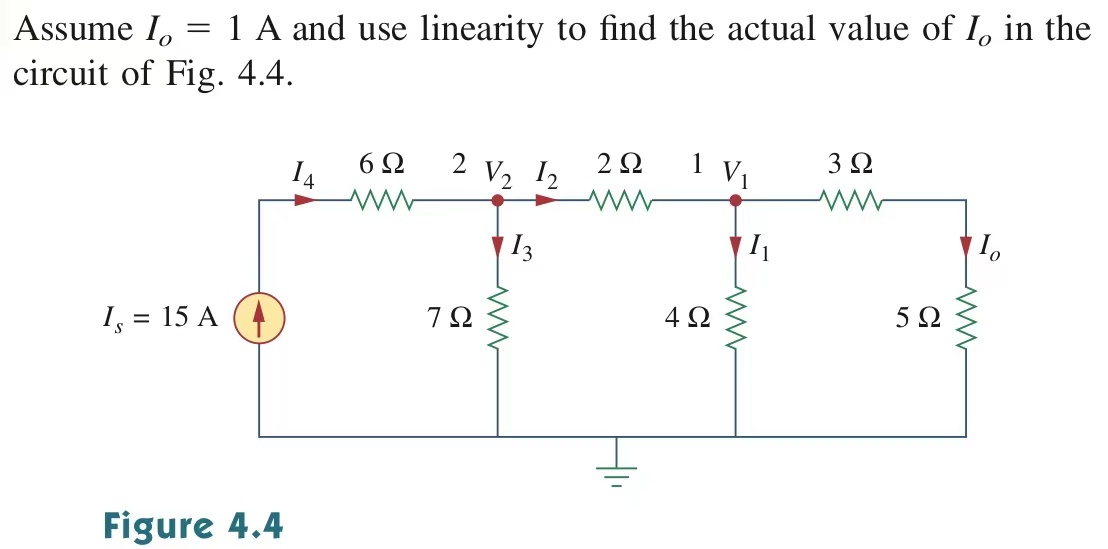
\includegraphics[scale=0.2]{img_cir/1.jpg}
\end{figure}
\end{frame}

%%%%%%%%%%%%%%%%%%%%%%%%%%%%%

\begin{frame}{Exercise}
\begin{figure}
\centering
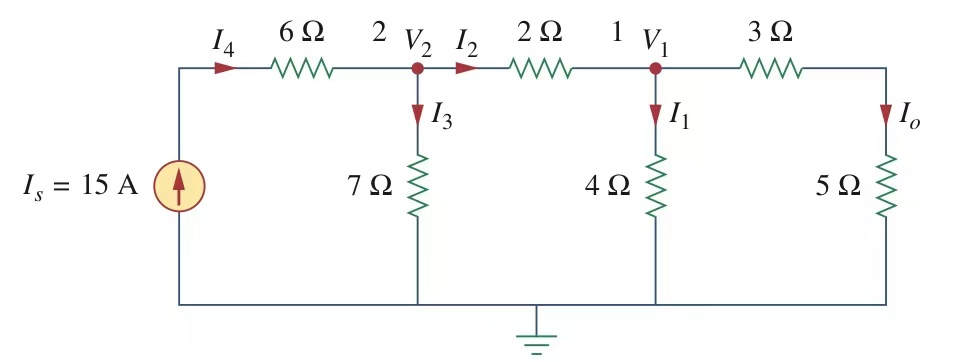
\includegraphics[scale=0.2]{img_cir/2.jpg}
\end{figure}
\textbf{Answer:} $I_0=3A$
\end{frame}

%%%%%%%%%%%%%%%%%%%%%%%%%%%%%

\begin{frame}{Superposition}
\textbf{Steps}
\newline
\begin{enumerate}
\item Only consider one \textbf{independent} source.
\begin{itemize}
\item voltage source: short circuit
\item current source: open circuit
\newline
\end{itemize}
\item Use additivity.
\end{enumerate}
\end{frame}

%%%%%%%%%%%%%%%%%%%%%%%%%%%%%

\begin{frame}{Exercise}
Find $i$ in the circuit.
\begin{figure}
\centering
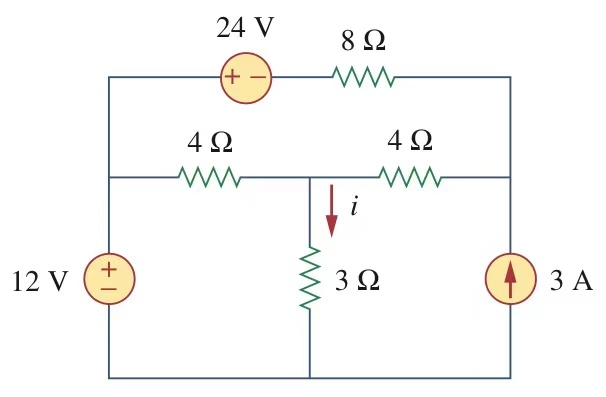
\includegraphics[scale=0.4]{img_cir/4.jpg}
\end{figure}
\end{frame}

%%%%%%%%%%%%%%%%%%%%%%%%%%%%%

\begin{frame}{Exercise}
\begin{figure}
\centering
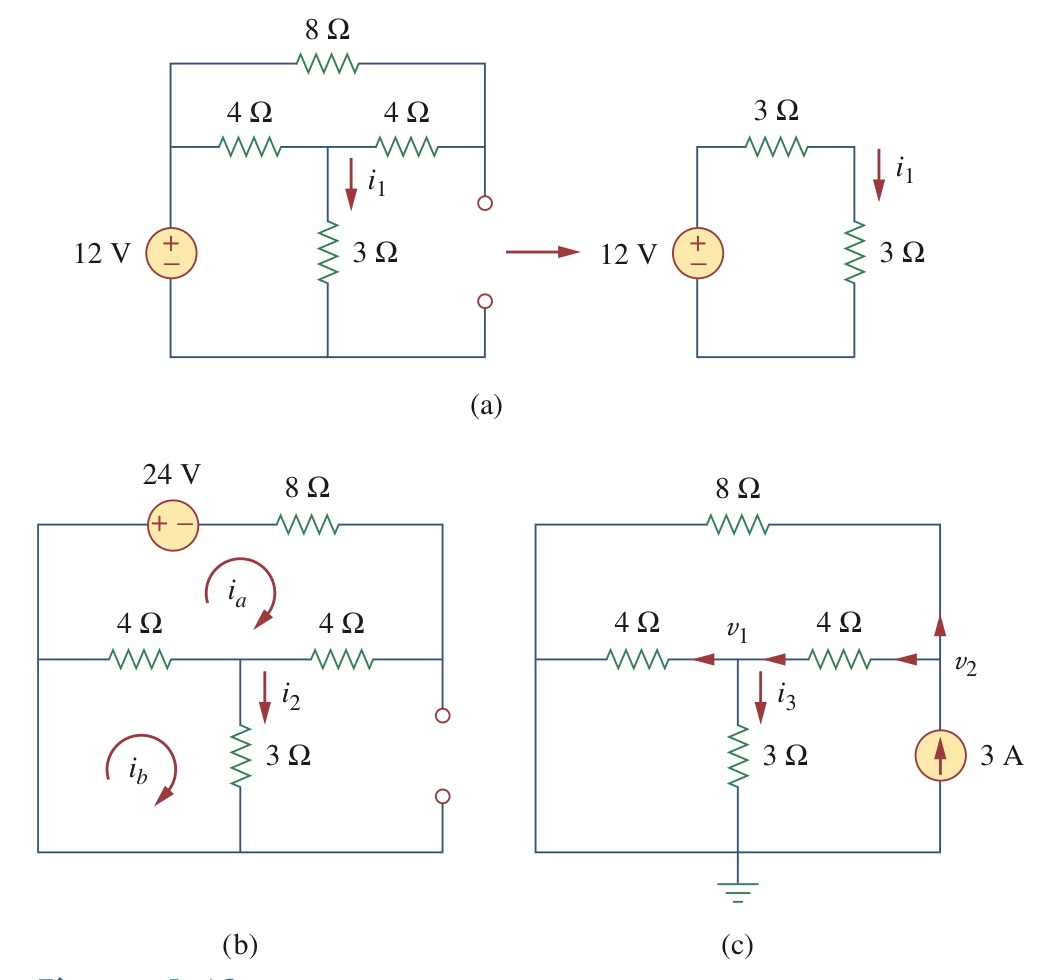
\includegraphics[scale=0.2]{img_cir/3.jpg}
\end{figure}
\textbf{Answer:} 2A
\end{frame}

%%%%%%%%%%%%%%%%%%%%%%%%%%%%%

\begin{frame}{Source Transformation}
We can replace a voltage source with a resistance with a
corresponding current source with the same resistance to simplify the circuit. 
\newline
In the case shown below, $v_s=i_s\times R$
\begin{figure}
\centering
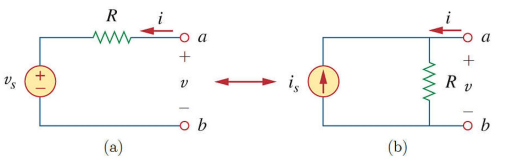
\includegraphics[scale=0.8]{img_cir/5.png}
\end{figure}
For dependent sources, the source transformation is also valid.

\end{frame}

%%%%%%%%%%%%%%%%%%%%%%%%%%%%%

\begin{frame}{Exercise}
Calculate $V_x$ in the circuit below by applying source transformation.

\begin{figure}
\centering
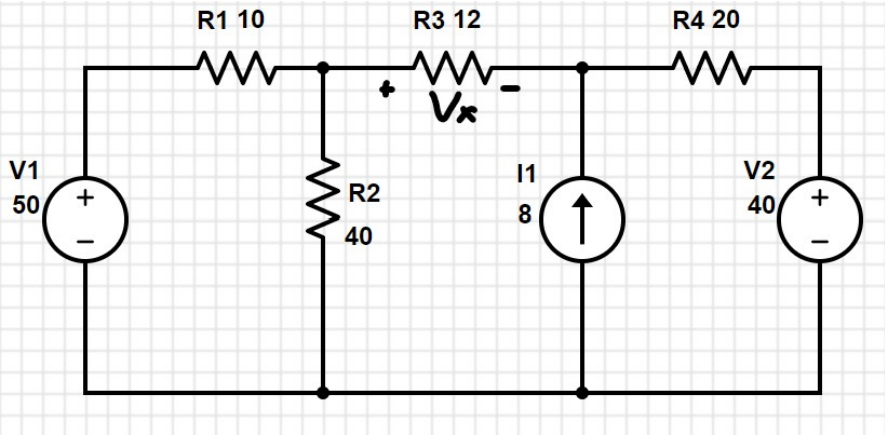
\includegraphics[scale=0.5]{img_cir/6.png}
\end{figure}
\end{frame}

%%%%%%%%%%%%%%%%%%%%%%%%%%%%%

\begin{frame}{Thevenin’s Theorem}
A linear two-terminal circuit can be replaced by an equivalent circuit consisting of a voltage source $V_{Th}$ in series with a resistor $R_{Th}$.

\begin{figure}
\centering
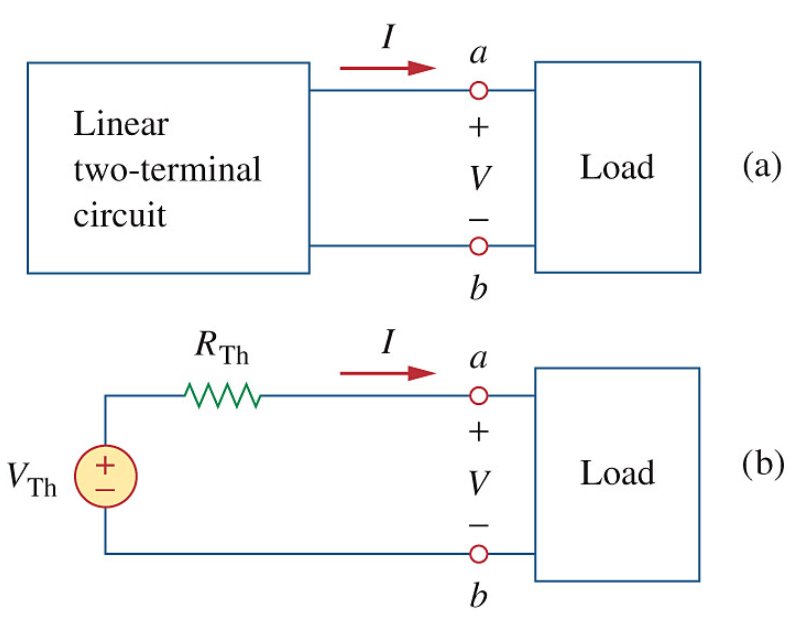
\includegraphics[scale=0.3]{img_cir/7.png}
\end{figure}

\begin{itemize}
\item $V_{Th}$: the open-circuit voltage at the terminals.
\item $R_{Th}$: the equivalent resistance at the terminals when all the \textcolor{red}{independent sources} are turned off.
\end{itemize}
\end{frame}

%%%%%%%%%%%%%%%%%%%%%%%%%%%%%

\begin{frame}{Exercise}
Obtain the Thevenin equivalent circuit of this circuit with respect to terminal a and b.
\begin{figure}
\centering
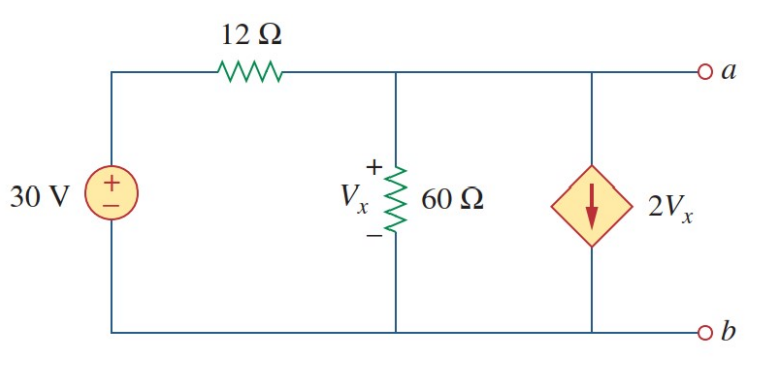
\includegraphics[scale=0.5]{img_cir/8.png}
\end{figure}
\end{frame}

%%%%%%%%%%%%%%%%%%%%%%%%%%%%%

\begin{frame}{Norton’s Theorem}
A linear two-terminal circuit can be replaced by an equivalent circuit consisting of a current source $I_{Th}$ in parallel with a resistor $R_{Th}$.

\begin{figure}
\centering
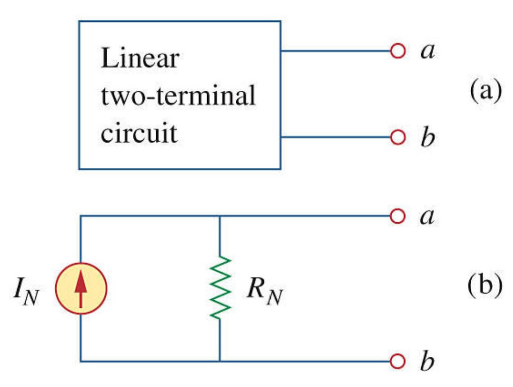
\includegraphics[scale=0.3]{img_cir/9.png}
\end{figure}

\begin{itemize}
\item $I_{Th}$: the short-circuit current at the terminals.
\item $R_{Th}$: the equivalent resistance at the terminals when all the \textcolor{red}{independent sources} are turned off.
\end{itemize}
\end{frame}

%%%%%%%%%%%%%%%%%%%%%%%%%%%%%

\begin{frame}{Exercise}
Obtain the Norton equivalent circuit of this circuit with respect to terminal a and b.
\begin{figure}
\centering
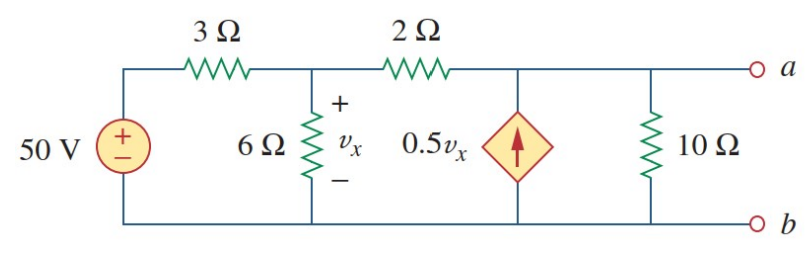
\includegraphics[scale=0.5]{img_cir/10.png}
\end{figure}
\end{frame}

%%%%%%%%%%%%%%%%%%%%%%%%%%%%%

\begin{frame}{Maximum Power Transfer}

A circuit is usually designed to provide power to a load. For different kinds of circuits, we have different concerns

\begin{itemize}
    \item \textbf{Maximum Power Efficiency:}
    In power utility systems, the amount of electricity is very large. Therefore, how to \textcolor{red}{ increase the efficiency of power transfer} becomes an important problem.
    \item \textbf{Maximum Power Transfer:}  In communication and instrumental systems, the amount of electricity is small so the problem of efficiency is not so important. Instead, we want to \textcolor{red}{transfer as much of power as possible to the load}.
\end{itemize}.


\end{frame}

%%%%%%%%%%%%%%%%%%%%%%%%%%%%%

\begin{frame}{Maximum Power Transfer}
 
The Thevenin’s equivalent circuit is useful in finding the maximum power delivered to a load. In the circuit below, $R_L$ represents the load.


\begin{figure}
\centering
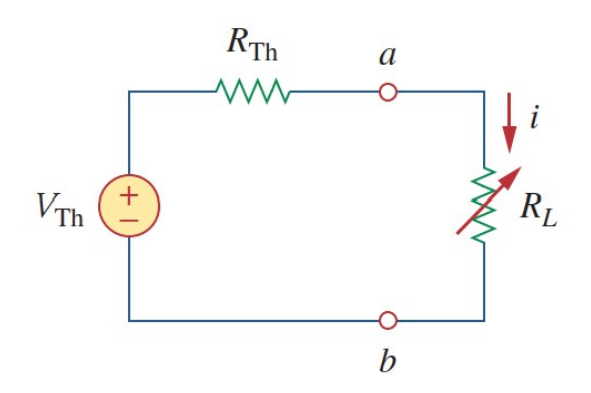
\includegraphics[scale=0.5]{img_cir/11.png}
\end{figure}

\end{frame}

%%%%%%%%%%%%%%%%%%%%%%%%%%%%%

\begin{frame}{Maximum Power Theorem}

Since
$$
    p=i^2R_{L}=\Big(\frac{V_{Th}}{R_{Th}+R_L}\Big)^2 R_{L} 
$$
Let $\frac{dP}{dR_L}=V_{Th}^2\frac{R_{Th}-R_L}{(R_{Th}+R_L)^3}=0$, we have $R_L=R_{Th}$.

And when $R_{L}=R_{Th}$, $\frac{d^2P}{dR_L^2}=V_{Th}^2\frac{2R_l-4R_{Th}}{(R_{Th}+R_L)^4}=-\frac{V_{Th}^2}{8R_{Th}^2}<0$.

Thus $p$ reaches maximum at $R_L=R_{Th}$. \textcolor{}{$p_{max}=\frac{V_{Th}^2}{4R_{Th}}$}

\end{frame}


%%%%%%%%%%%%%%%%%%%%%%%%%%%%%%%%%%%%%%%%%%%%%%%%%%%
% OP-AMP
\section{Operational Amplifiers}

%%%%%%%%%%%%%%%%%%%%%%%%%%%%%
\begin{frame}{Operational Amplifiers}

Definition: an circuit element that can
\begin{itemize}
    \item amplify an input electrical signal
    \item perform mathematical operations (e.g. $+$, $-$, $\times$, $\div$) on this signal when combined with feedback circuits
\end{itemize}


\begin{multicols}{2}
    \sectiont{}
    \begin{figure}[H]
        \centering
        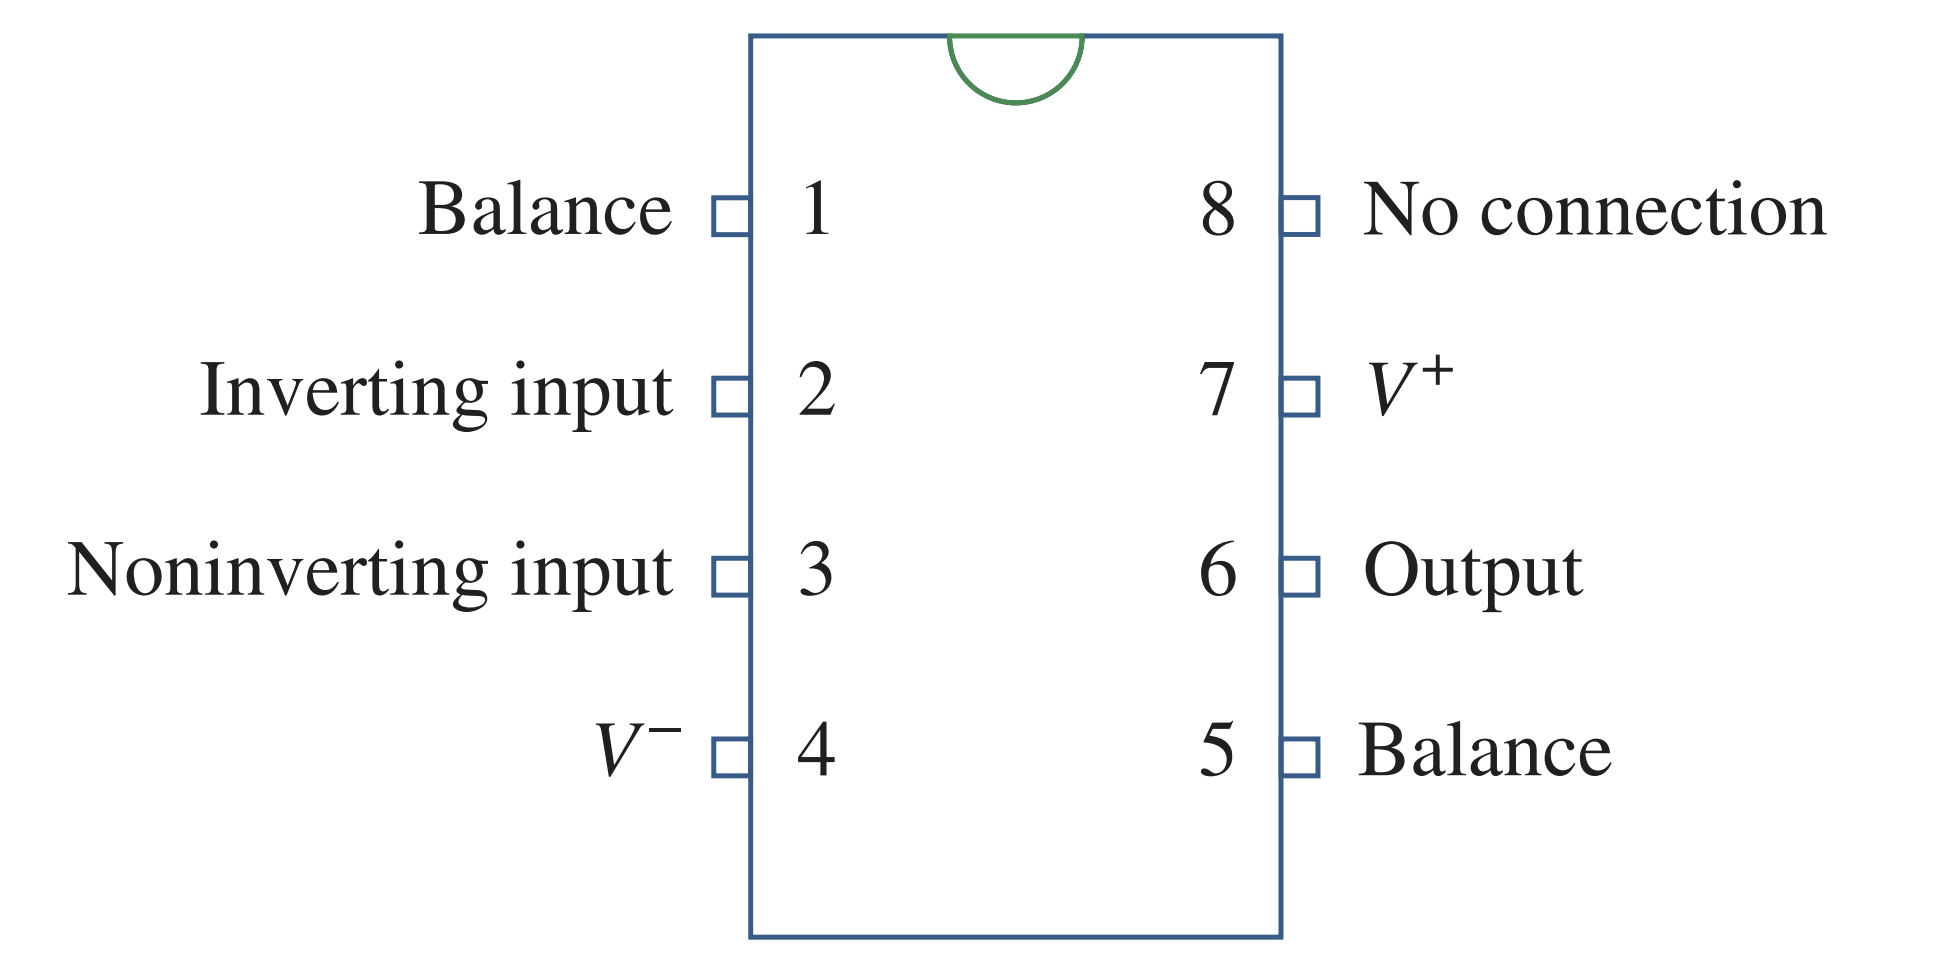
\includegraphics[width=0.47\textwidth]{img_opamp/1_opamp structure.png}
        \caption{Structure of op-amp}
    \end{figure}
    \sectiont{}
    \begin{figure}[H]
        \centering
        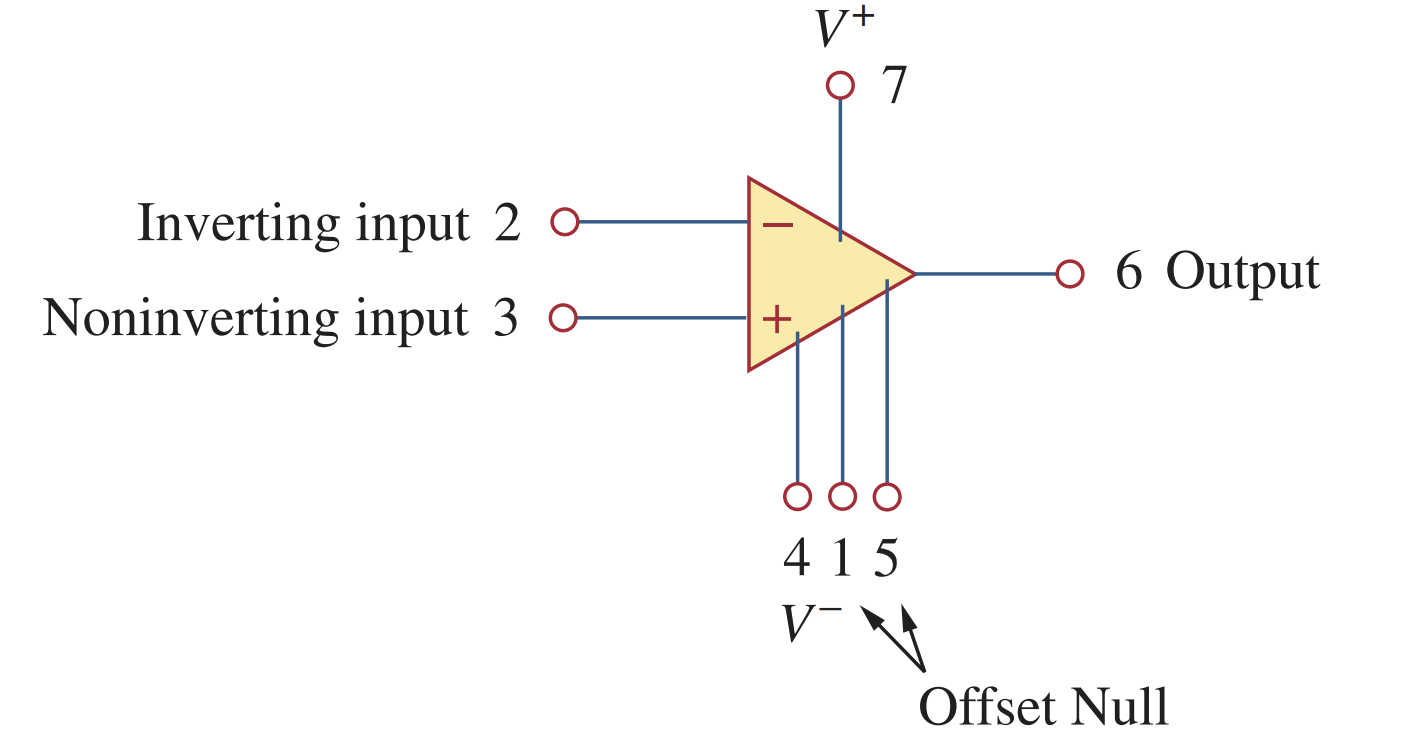
\includegraphics[width=0.45\textwidth]{img_opamp/2_opamp connection.png}
        \caption{Symbol of op-amp}
    \end{figure}
    
\end{multicols}


\end{frame}

%%%%%%%%%%%%%%%%%%%%%%%%%%%%%
\begin{frame}{Operational Amplifiers}


Limitation: the magnitude of the output voltage cannot be as large as we want
\begin{itemize}
    \item It cannot exceed the supply power $V^{+}$
    \item Otherwise: saturation
    \item \textbf{Ignored in ideal op-amps}
\end{itemize}
\begin{figure}[H]
    \centering
    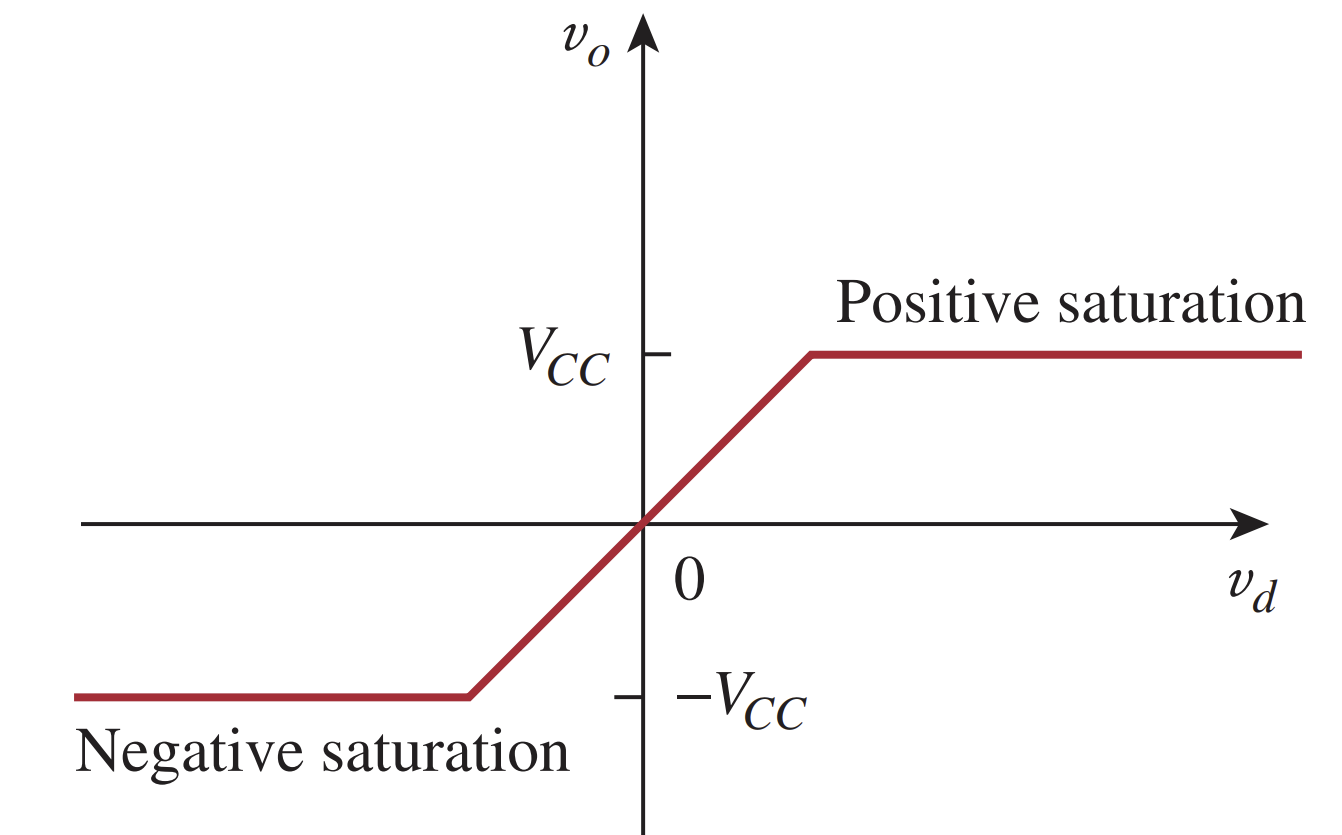
\includegraphics[width=0.5\textwidth]{img_opamp/13_saturation.png}
    \caption{Saturation}
\end{figure}

\end{frame}


%%%%%%%%%%%%%%%%%%%%%%%%%%%%%
\begin{frame}{Ideal Op-amp}

Assumption:
\begin{itemize}
    \item Infinite open-loop gain ($A = \infty$)
    \item Infinite input resistance ($R_i = \infty$)
    \item Zero output resistance ($R_0 = 0$)
    \item (Does not mean that $v_0 = \infty$)
\end{itemize}

\begin{multicols}{2}
    \sectiont{}
    \begin{figure}[H]
        \centering
        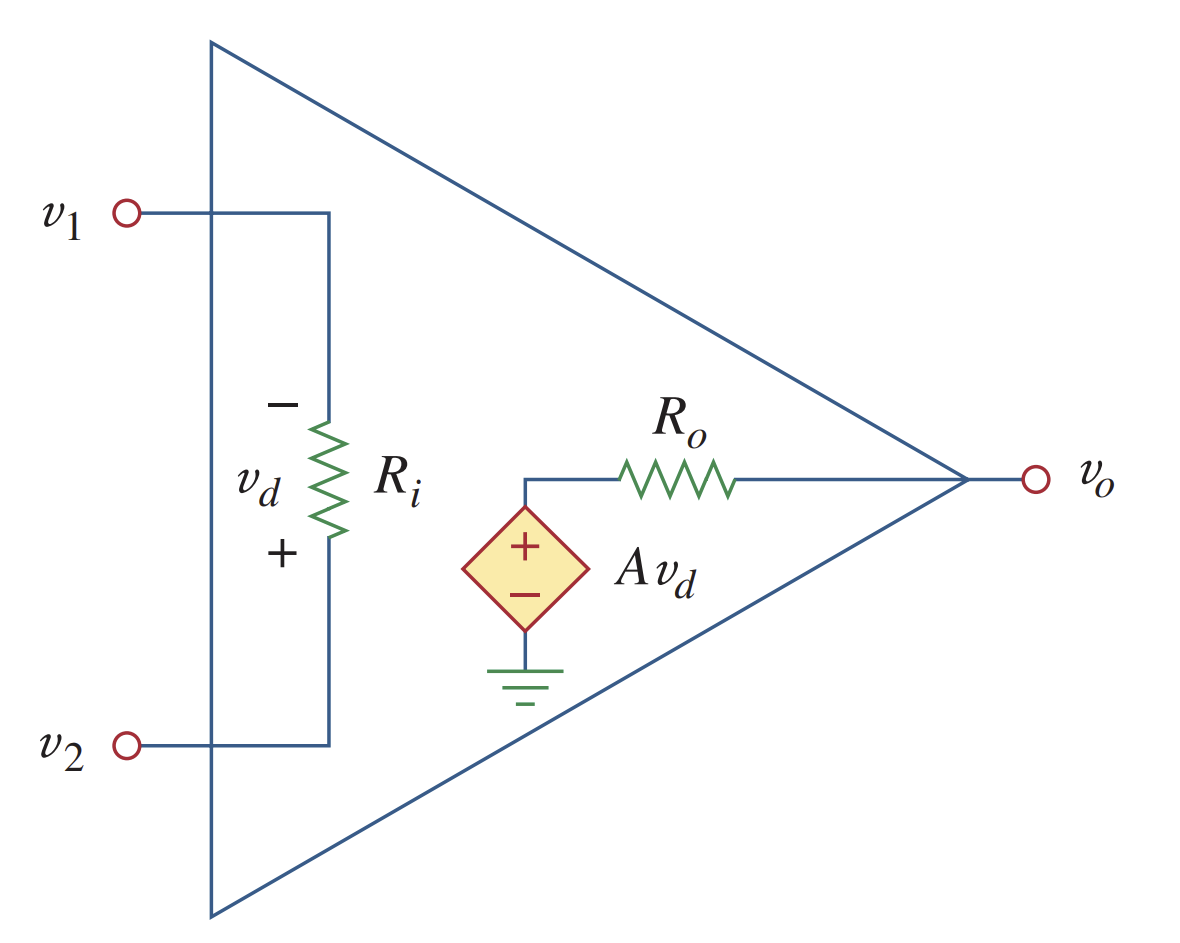
\includegraphics[width=0.35\textwidth]{img_opamp/3_opamp equivalent.png}
        \caption{Op-amp's equivalent circuit}
    \end{figure}
    \sectiont{}
    \begin{figure}[H]
        \centering
        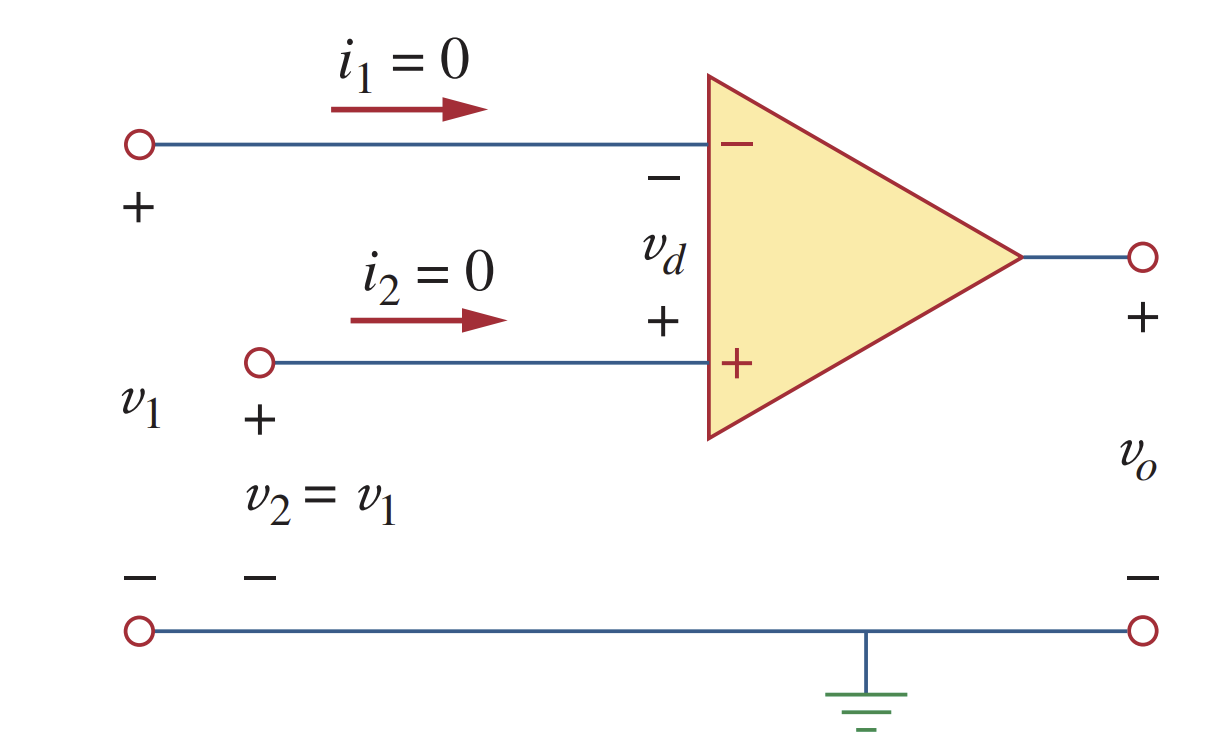
\includegraphics[width=0.46\textwidth]{img_opamp/4_ideal op amp.png}
        \caption{Symbol of ideal op-amp}
    \end{figure}
    
\end{multicols}

    
\end{frame}

%%%%%%%%%%%%%%%%%%%%%%%%%%%%%
\begin{frame}{Ideal Op-amp}

Characteristics of ideal op-amp:
\begin{itemize}
    \item Open circuit at two input terminals ($i_1 = i_2 = 0$)
    \item Same voltage at two input terminals ($v_1 = v_2$)
    \item (\textbf{Does not mean that $i_o = 0$!})
\end{itemize}

\begin{multicols}{2}
    \sectiont{}
    \begin{figure}[H]
        \centering
        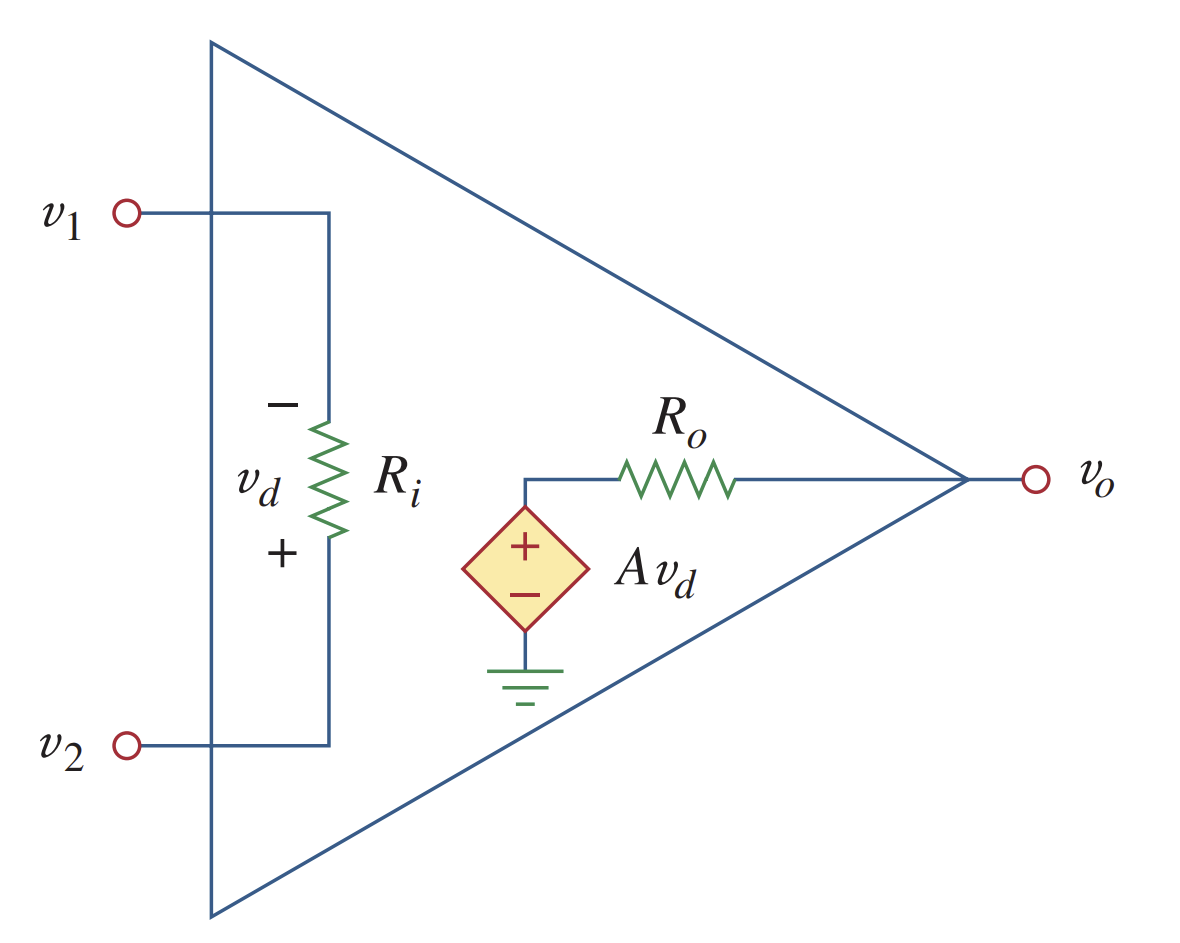
\includegraphics[width=0.35\textwidth]{img_opamp/3_opamp equivalent.png}
        \caption{Op-amp's equivalent circuit}
    \end{figure}
    \sectiont{}
    \begin{figure}[H]
        \centering
        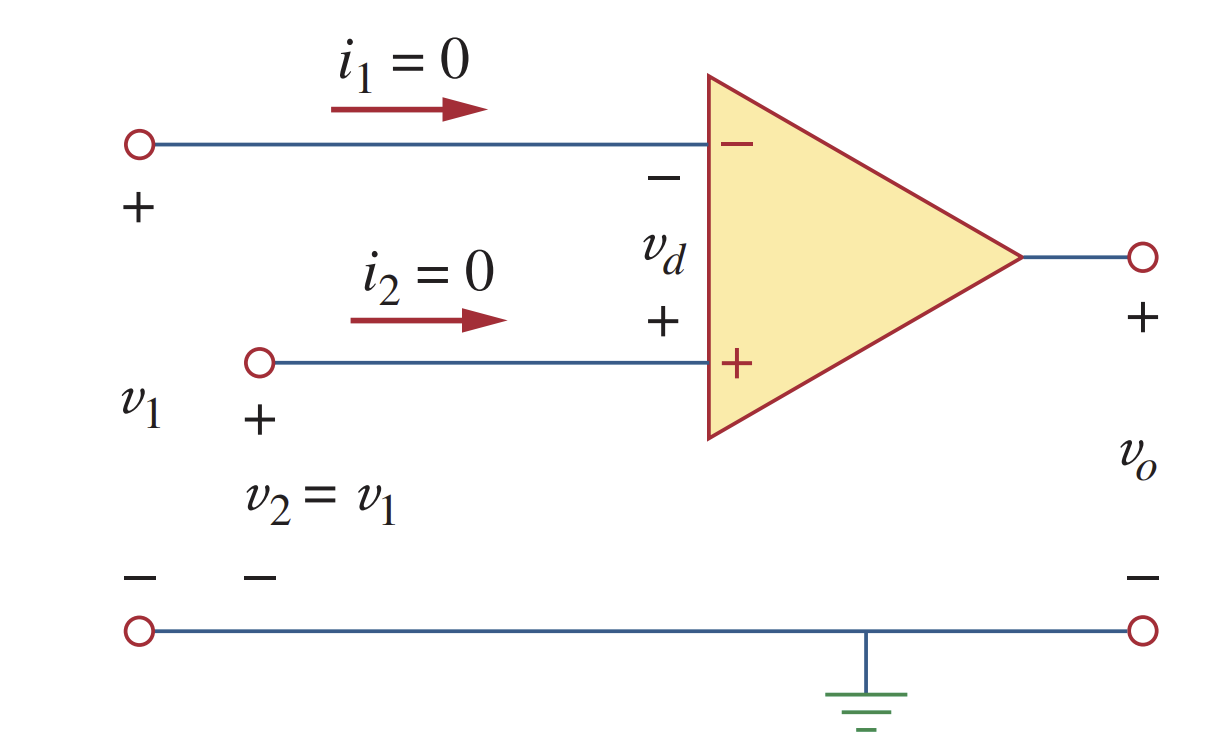
\includegraphics[width=0.46\textwidth]{img_opamp/4_ideal op amp.png}
        \caption{Symbol of ideal op-amp}
    \end{figure}
    
\end{multicols}
    
\end{frame}

%%%%%%%%%%%%%%%%%%%%%%%%%%%%%
\begin{frame}{Basic Op-amp Circuits: Inverting Op-amp}

\begin{multicols}{2}
    \sectiont{}
    Open-loop gain:
    $$A = \frac{v_0}{v_i} = -\frac{R_f}{R_1}$$
    Deduction:
    $$\left\{\begin{aligned}
        &\frac{v_i-v_1}{R_1} = \frac{v_1 - v_o}{R_f}\\
        &v_1 = v_2 = 0\\
    \end{aligned}\right.
    $$
    
    \sectiont{}
    \begin{figure}[H]
        \centering
        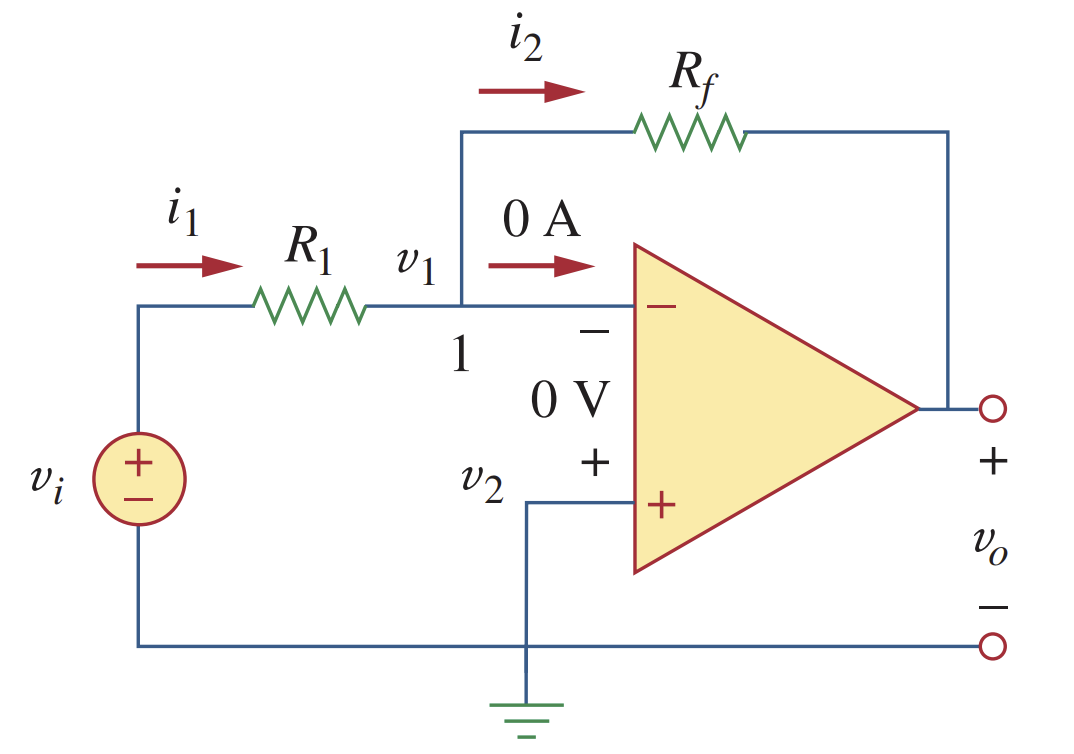
\includegraphics[width=0.45\textwidth]{img_opamp/5_ inverting.png}
        \caption{Inverting op-amp}
    \end{figure}
\end{multicols}

An interesting variant:
%TODO: 一张图片


\end{frame}

%%%%%%%%%%%%%%%%%%%%%%%%%%%%%
\begin{frame}{Basic Op-amp Circuits: Non-inverting Op-amp}

\begin{multicols}{2}
    \sectiont{}
    Open-loop gain:
    $$A = \frac{v_0}{v_i} = 1 + \frac{R_f}{R_1}$$
    Deduction:
    $$\left\{\begin{aligned}
        &\frac{0 - v_1}{R_1} = \frac{v_1-v_o}{R_f}\\
        &v_1=v_2=v_i\\
    \end{aligned}\right.
    $$
    
    \sectiont{}
    \begin{figure}[H]
        \centering
        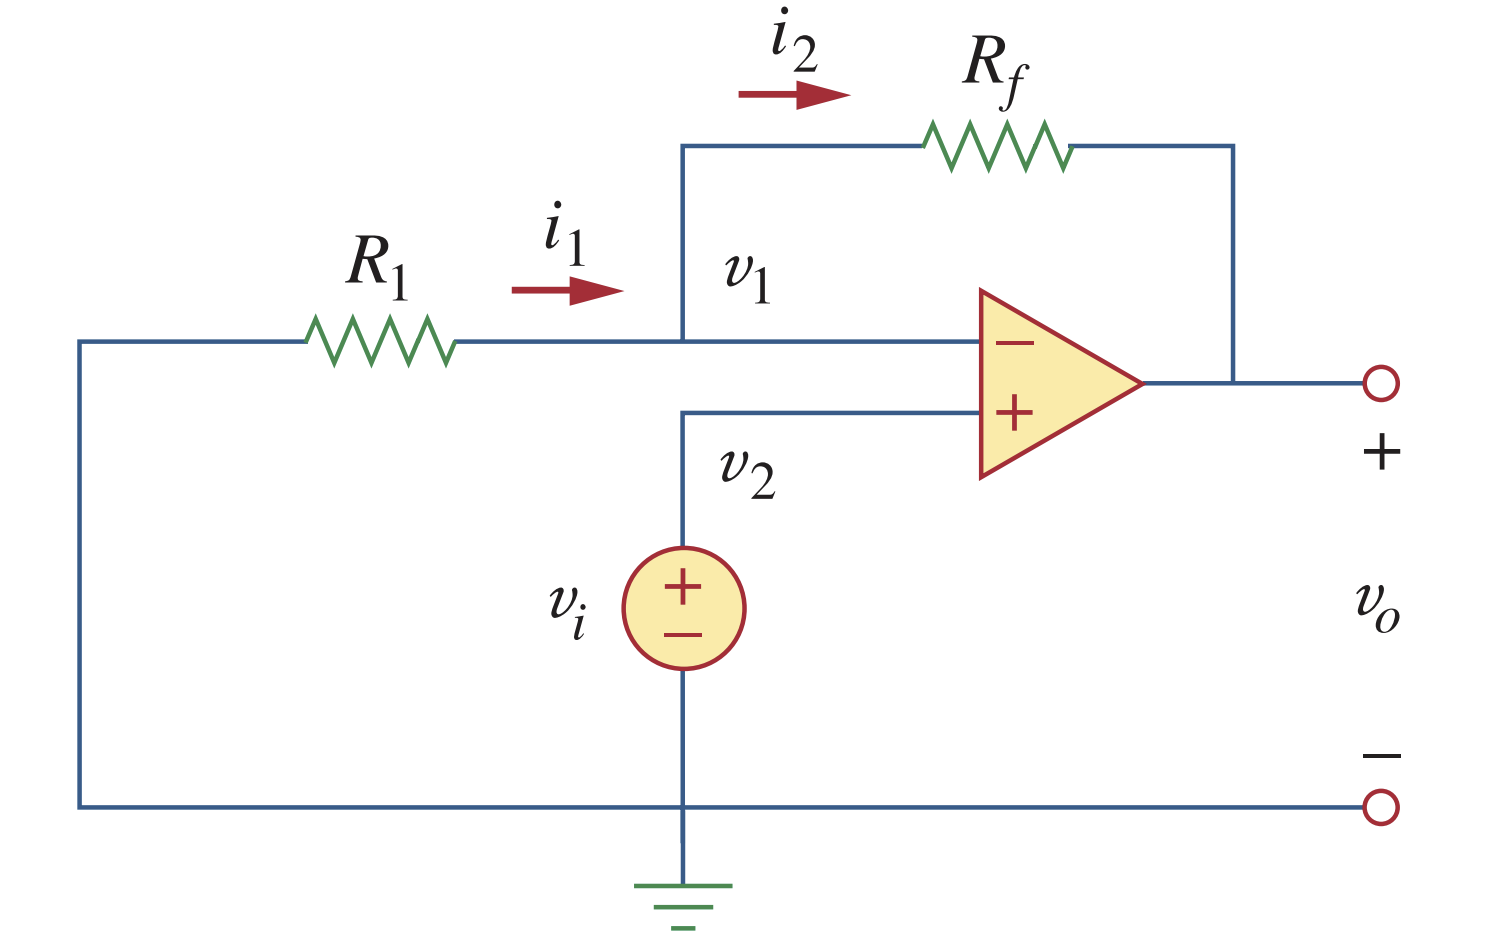
\includegraphics[width=0.45\textwidth]{img_opamp/6_non-inverting.png}
        \caption{Non-inverting op-amp}
    \end{figure}
\end{multicols}

\begin{multicols}{2}
    \sectiont{}
    A variant: voltage follower
    \begin{itemize}
        \item $v_o=v_i$
        \item Let $R_f=0$ or $R_1 = \infty$
        \item Isolate two parts of circuits
        \item Decrease inter-stage loads
    \end{itemize}
    
    \sectiont{}
    \begin{figure}[H]
        \centering
        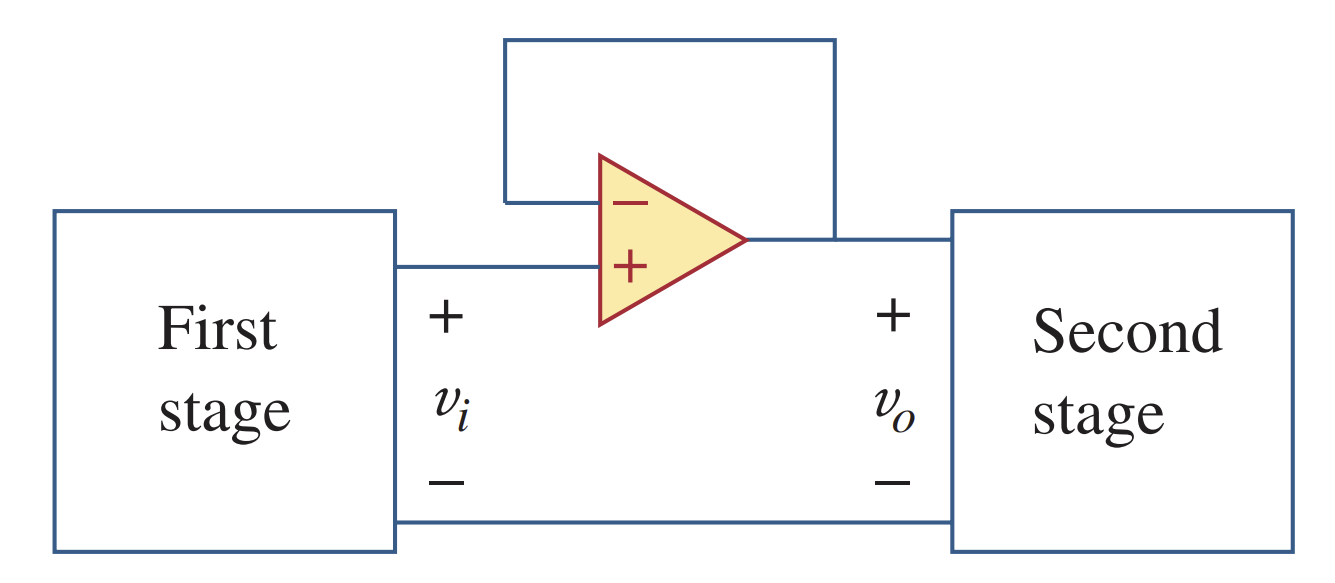
\includegraphics[width=0.45\textwidth]{img_opamp/7_voltage follower.png}
        \caption{Voltage follower}
    \end{figure}
    
\end{multicols}

\end{frame}

%%%%%%%%%%%%%%%%%%%%%%%%%%%%%
\begin{frame}{Basic Op-amp Circuits: Summing Op-amp}

\begin{multicols}{2}
    \sectiont{}
    Input-output relationship:
    $$v_o = -(\frac{R_f}{R_1}v_1 + \frac{R_f}{R_2}v_2 + \frac{R_f}{R_3}v_3)$$
    Notes:
    \begin{itemize}
        \item Be aware of the minus sign, summing and also inverting
        \item Treat it as a advanced version of inverting op-amp
    \end{itemize}
    
    \sectiont{}
    \begin{figure}[H]
        \centering
        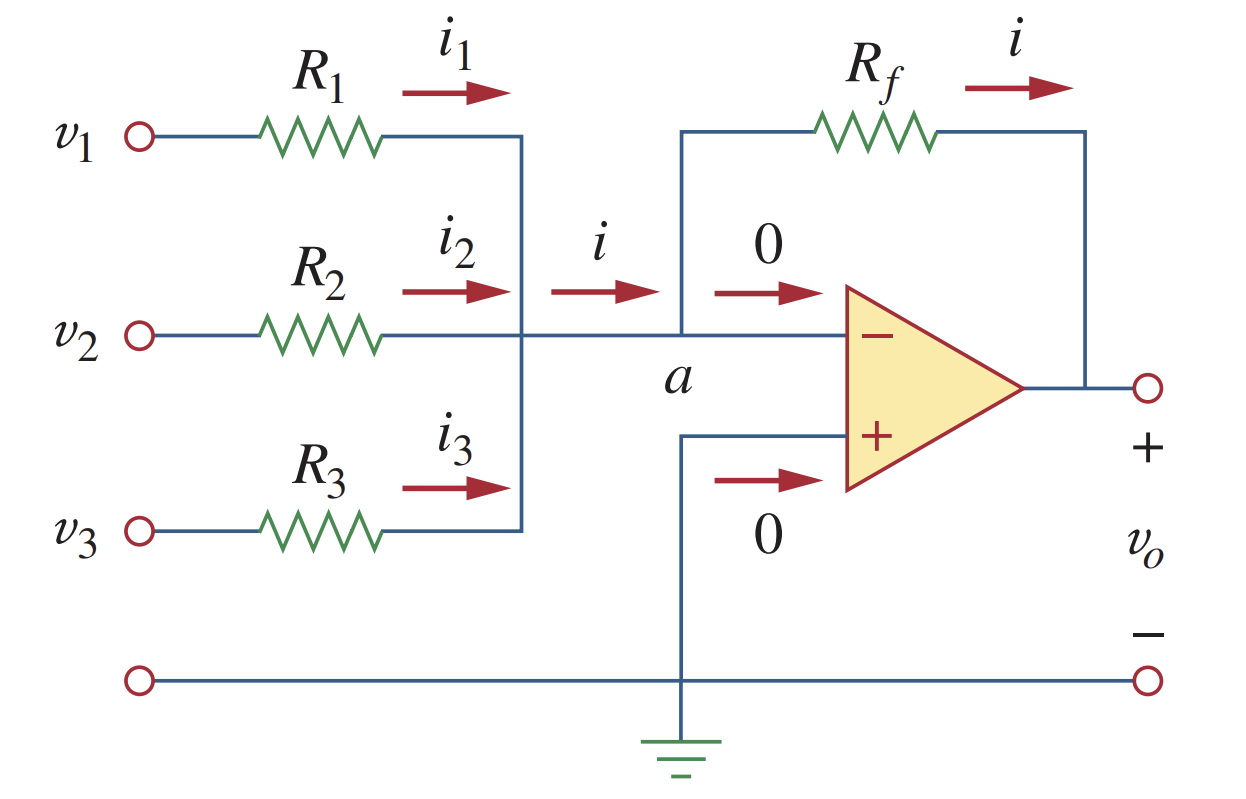
\includegraphics[width=0.5\textwidth]{img_opamp/8_adder.png}
        \caption{Summing op-amp}
    \end{figure}
\end{multicols}

Special cases:
\begin{itemize}
    \item $R_1 = R_2 = R_3 = R \Rightarrow v_o = -\frac{R_f}{R}(v_1+v_2+v_3)$
    \item $R_1=R_2=R_3=R_f=R \Rightarrow v_o = -(v_1+v_2+v_3)$
\end{itemize}
    
\end{frame}

%%%%%%%%%%%%%%%%%%%%%%%%%%%%%
\begin{frame}{Basic Op-amp Circuits: Difference Op-amp}

\begin{figure}[H]
    \centering
    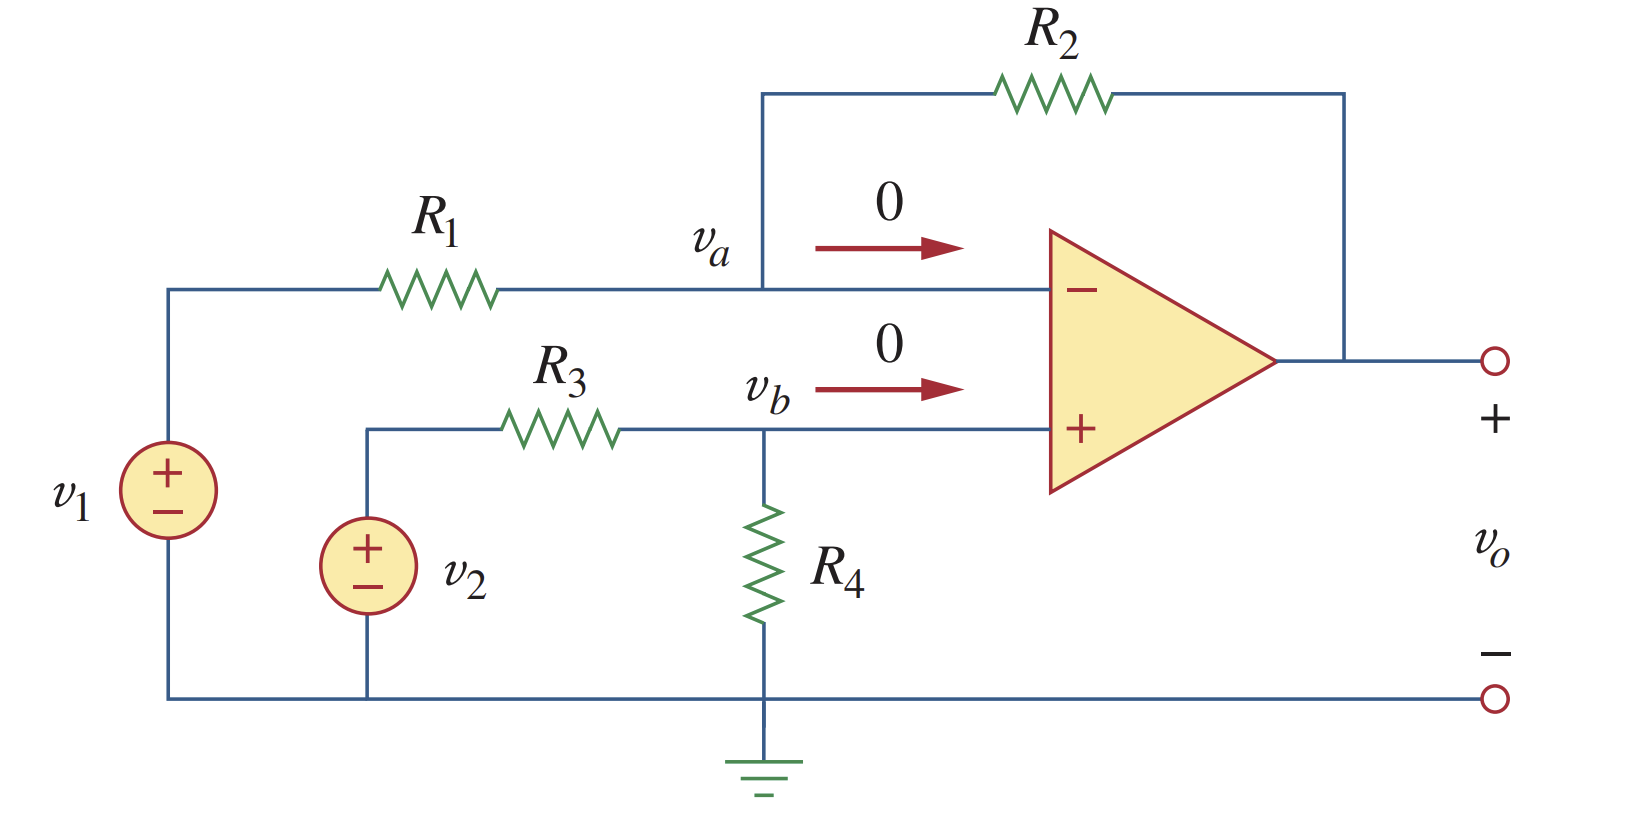
\includegraphics[width=0.5\textwidth]{img_opamp/9_difference.png}
    \caption{Difference op-amp}
\end{figure}
Input-output relationship:
$$v_o = \left[ (\frac{R_2}{R_1}+1)(\frac{R_4/R_3}{1+R_4/R_3})\right]v_2 - \left[\frac{R_2}{R_1}\right]v_1$$
Special cases:
\begin{itemize}
    \item $\frac{R_1}{R_2}=\frac{R_3}{R_4} \Rightarrow v_o = \frac{R_2}{R_1}(v_2-v_1)$
    \item $R_1 = R_2, R_3 = R_4 \Rightarrow v_o = v_2-v_1$
\end{itemize}

    
\end{frame}


%%%%%%%%%%%%%%%%%%%%%%%%%%%%%
\begin{frame}{Cascaded Op-amp Circuits}
\begin{figure}[H]
    \centering
    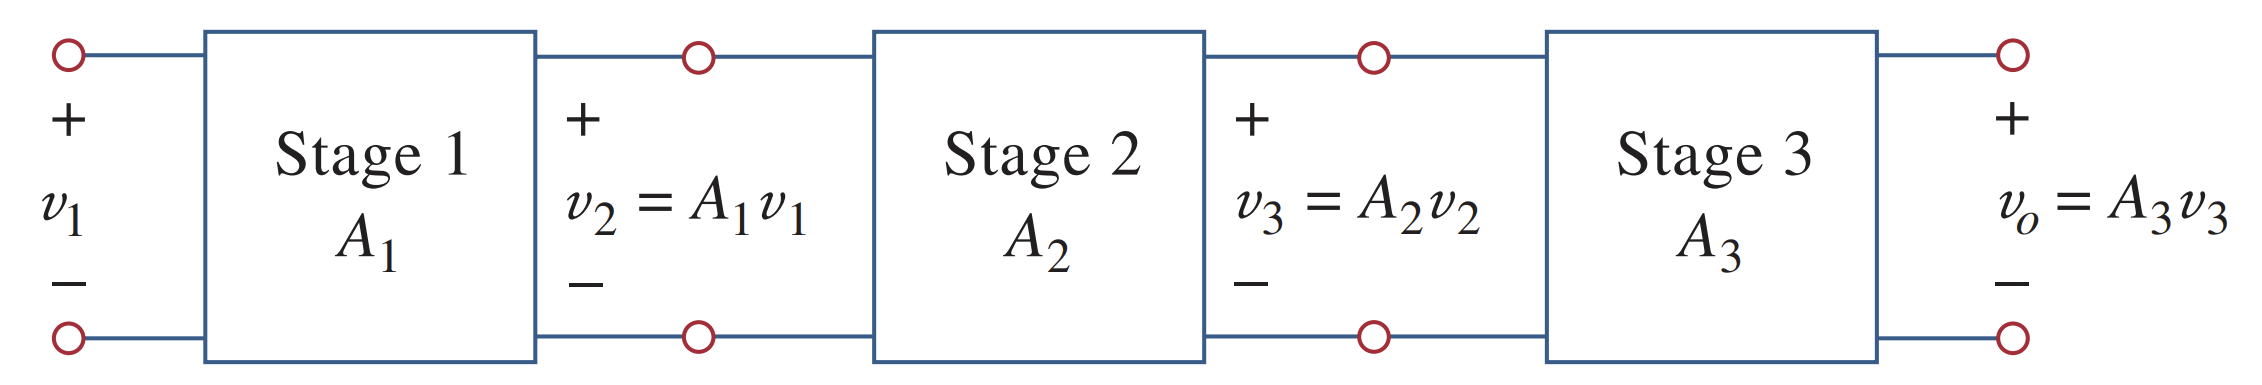
\includegraphics[width=0.9\textwidth]{img_opamp/10_cascaded.png}
    \caption{Cascaded op-amp circuits}
\end{figure}

$$A_{total} =\frac{v_2}{v_1}\frac{v_3}{v_2}\frac{v_o}{v_1} =  A_1A_2A_3$$

    
\end{frame}

%%%%%%%%%%%%%%%%%%%%%%%%%%%%%
\begin{frame}{Basic Op-amp Circuits: Summary}
For basic op-amp circuits:
\begin{table}[]
    \centering
    \begin{tabular}{cc}
        \toprule
        Op-amp circuits & Input-output relationship\\
        \midrule
        Inverting amplifier & $A = \frac{v_0}{v_i} = -\frac{R_f}{R_1}$\\
        Non-inverting amplifier & $A = \frac{v_0}{v_i} = 1 + \frac{R_f}{R_1}$\\
        Voltage follower & $v_o=v_i$\\
        Summing amplifier & $v_o = -(\frac{R_f}{R_1}v_1 + \frac{R_f}{R_2}v_2 + \frac{R_f}{R_3}v_3)$\\
        Difference amplifier & $v_o = \left[ (\frac{R_2}{R_1}+1)(\frac{R_4/R_3}{1+R_4/R_3})\right]v_2 - \left[\frac{R_2}{R_1}\right]v_1$\\
        \bottomrule
    \end{tabular}
\end{table}

For complicated op-amp circuits:
\begin{itemize}
    \item Identify basic op-amp circuits within it
    \item Use the formula for cascaded op-amp circuit
    \item Be proficient in listing nodal analysis equations to obtain $v_o/v_i$
\end{itemize}
    
\end{frame}

%%%%%%%%%%%%%%%%%%%%%%%%%%%%%
\begin{frame}{Application: Digital-to-Analog Converter converter}

\begin{figure}[H]
    \centering
    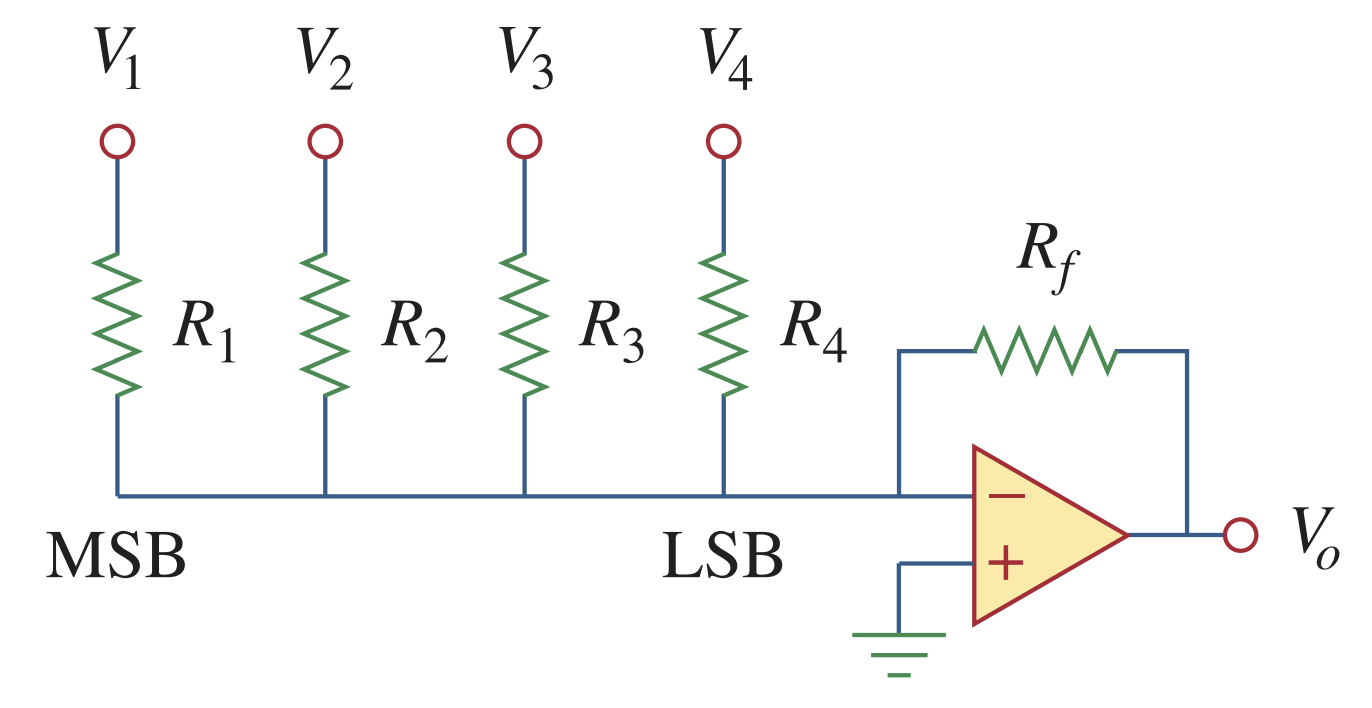
\includegraphics[width=0.4\textwidth]{img_opamp/11_converter.png}
    \caption{Circuit of D2A converter}
\end{figure}

Input $V_1, V_2, V_3, V_4$ takes only 0 or 1.

Resistors satisfy $R_4 = 2R_3, R_3 = 2R_2, R_2=2R_1$.

$$V_o = c(8V_1+4V_2+2V_3+V_4)$$

$V_o$ is propositional to the binary representation $\left[V_1V_2V_3V_4\right]$.

\end{frame}

%%%%%%%%%%%%%%%%%%%%%%%%%%%%%
\begin{frame}{Exercise}
For the circuit below, find $v_o$.

Hint: cascading of basic op-amp circuits
\begin{figure}[H]
    \centering
    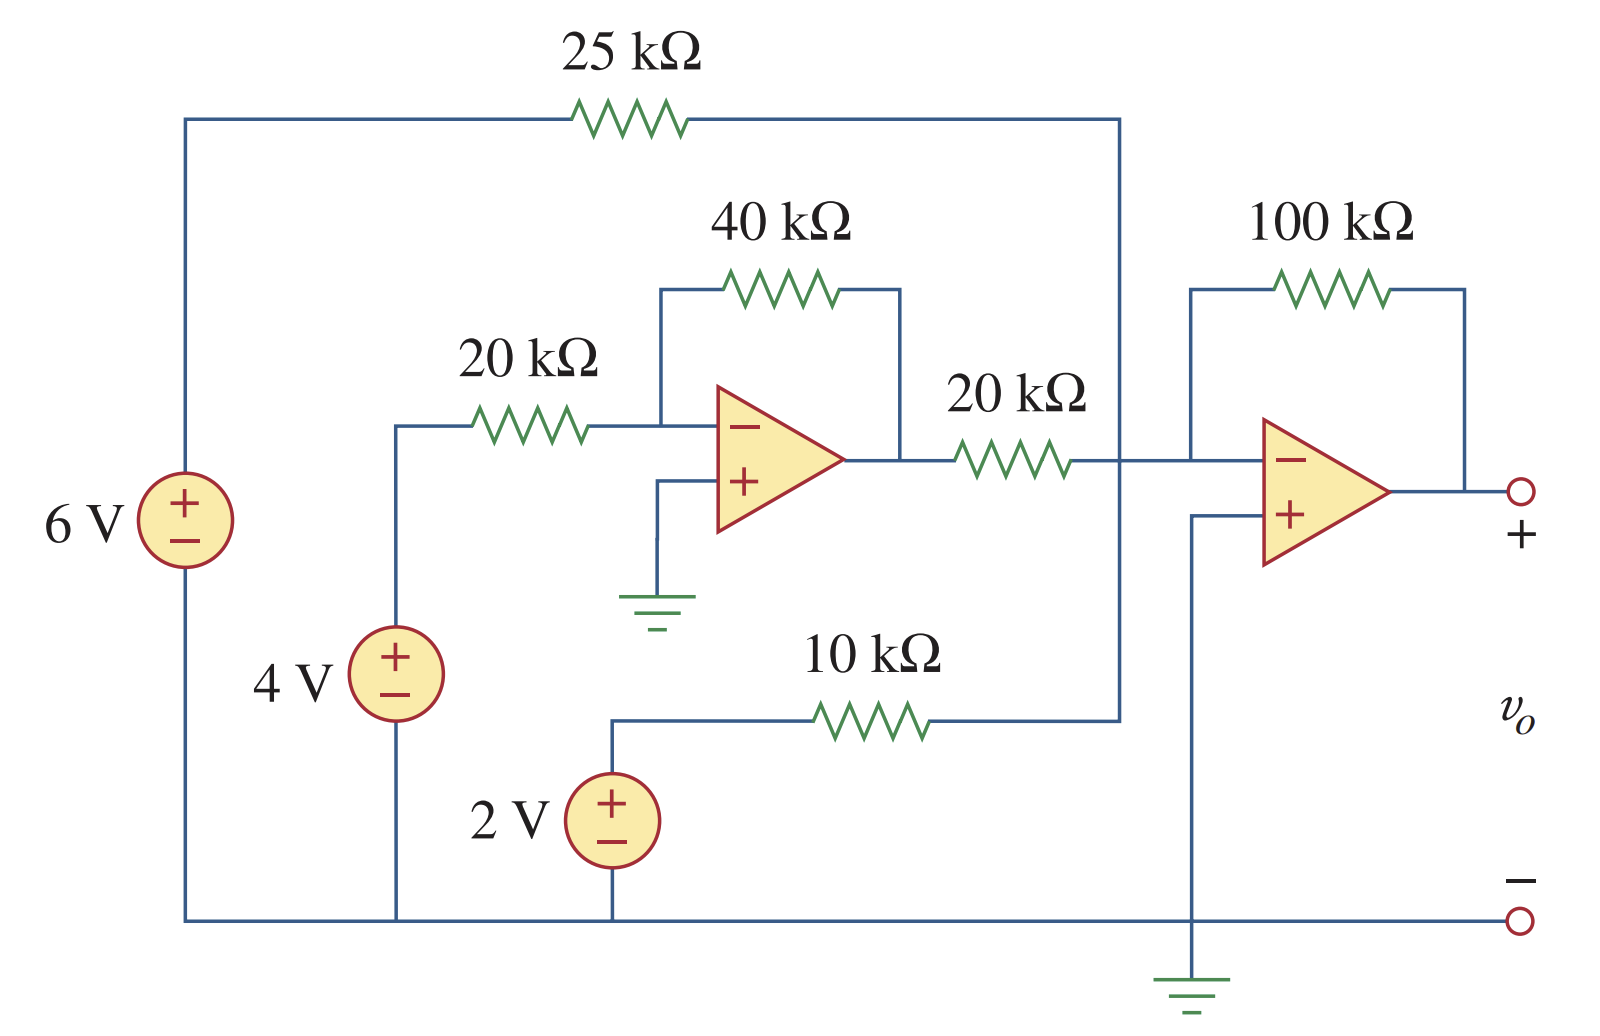
\includegraphics[width=0.8\textwidth]{img_opamp/exercise.png}
\end{figure}
    
\end{frame}

%%%%%%%%%%%%%%%%%%%%%%%%%%%%%
\begin{frame}{Exercise}
\begin{figure}[H]
    \centering
    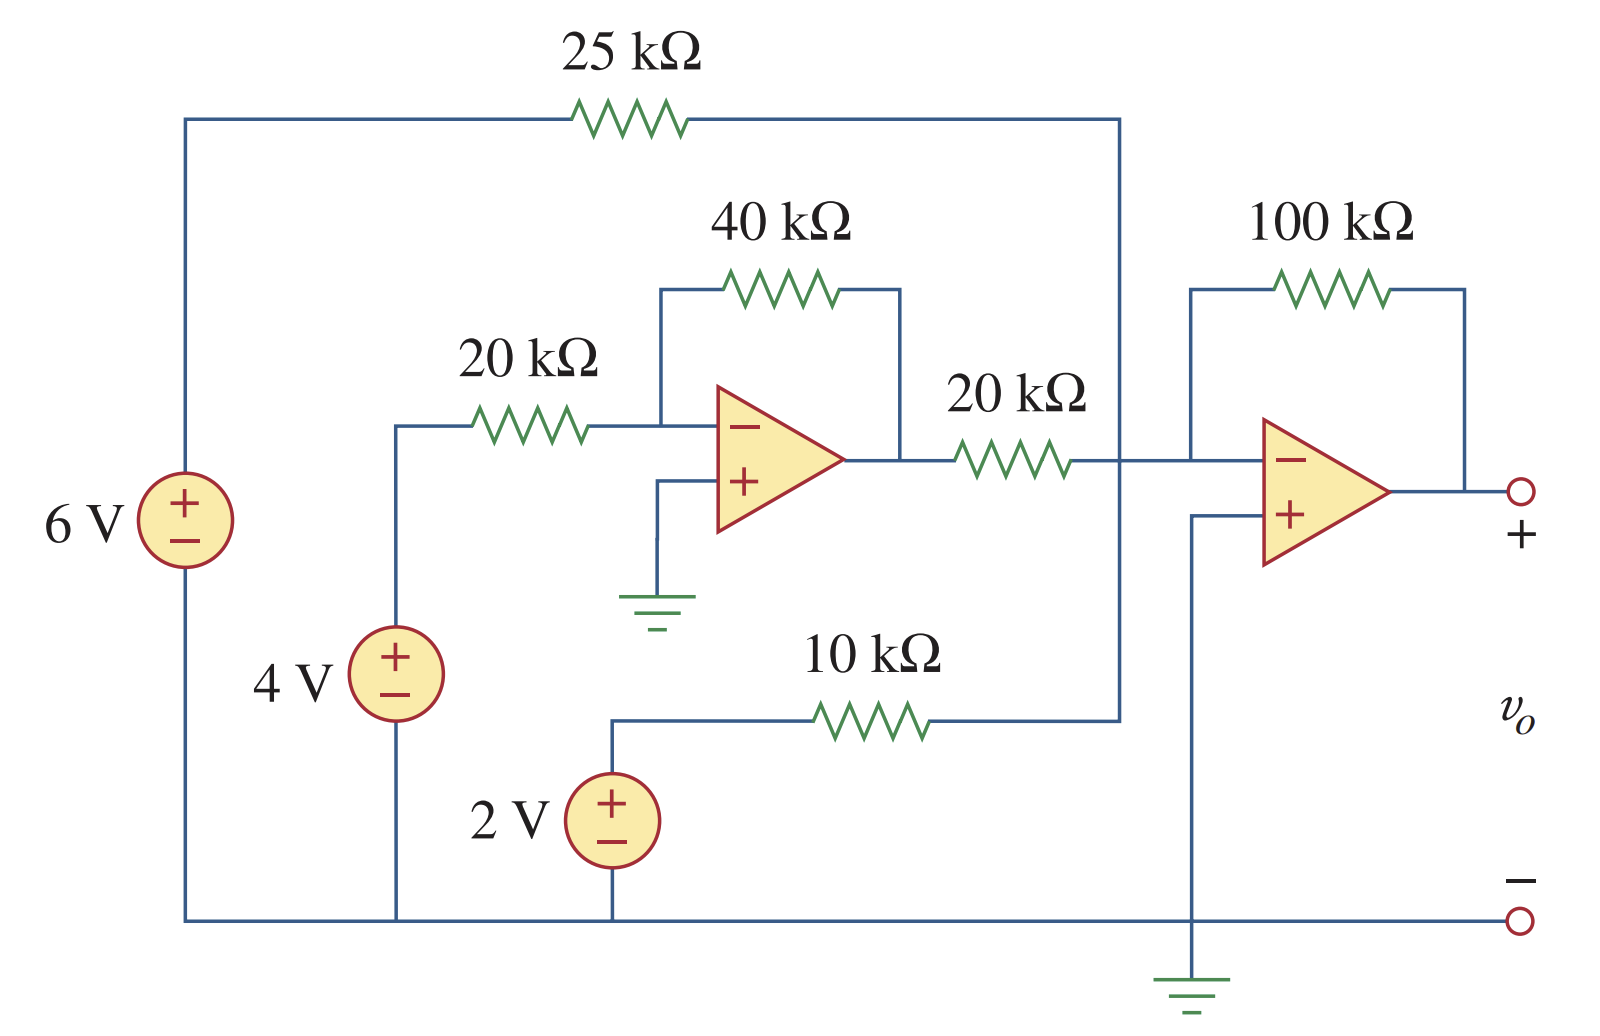
\includegraphics[width=0.65\textwidth]{img_opamp/exercise.png}
\end{figure}
Answer: $-4\text{V}$
    
\end{frame}

%%%%%%%%%%%%%%%%%%%%%%%%%%%%%
\begin{frame}{Exercise}
Determine the gain $v_o/v_i$ of the circuit below.

Hint: list the equations yourself!
\begin{figure}[H]
    \centering
    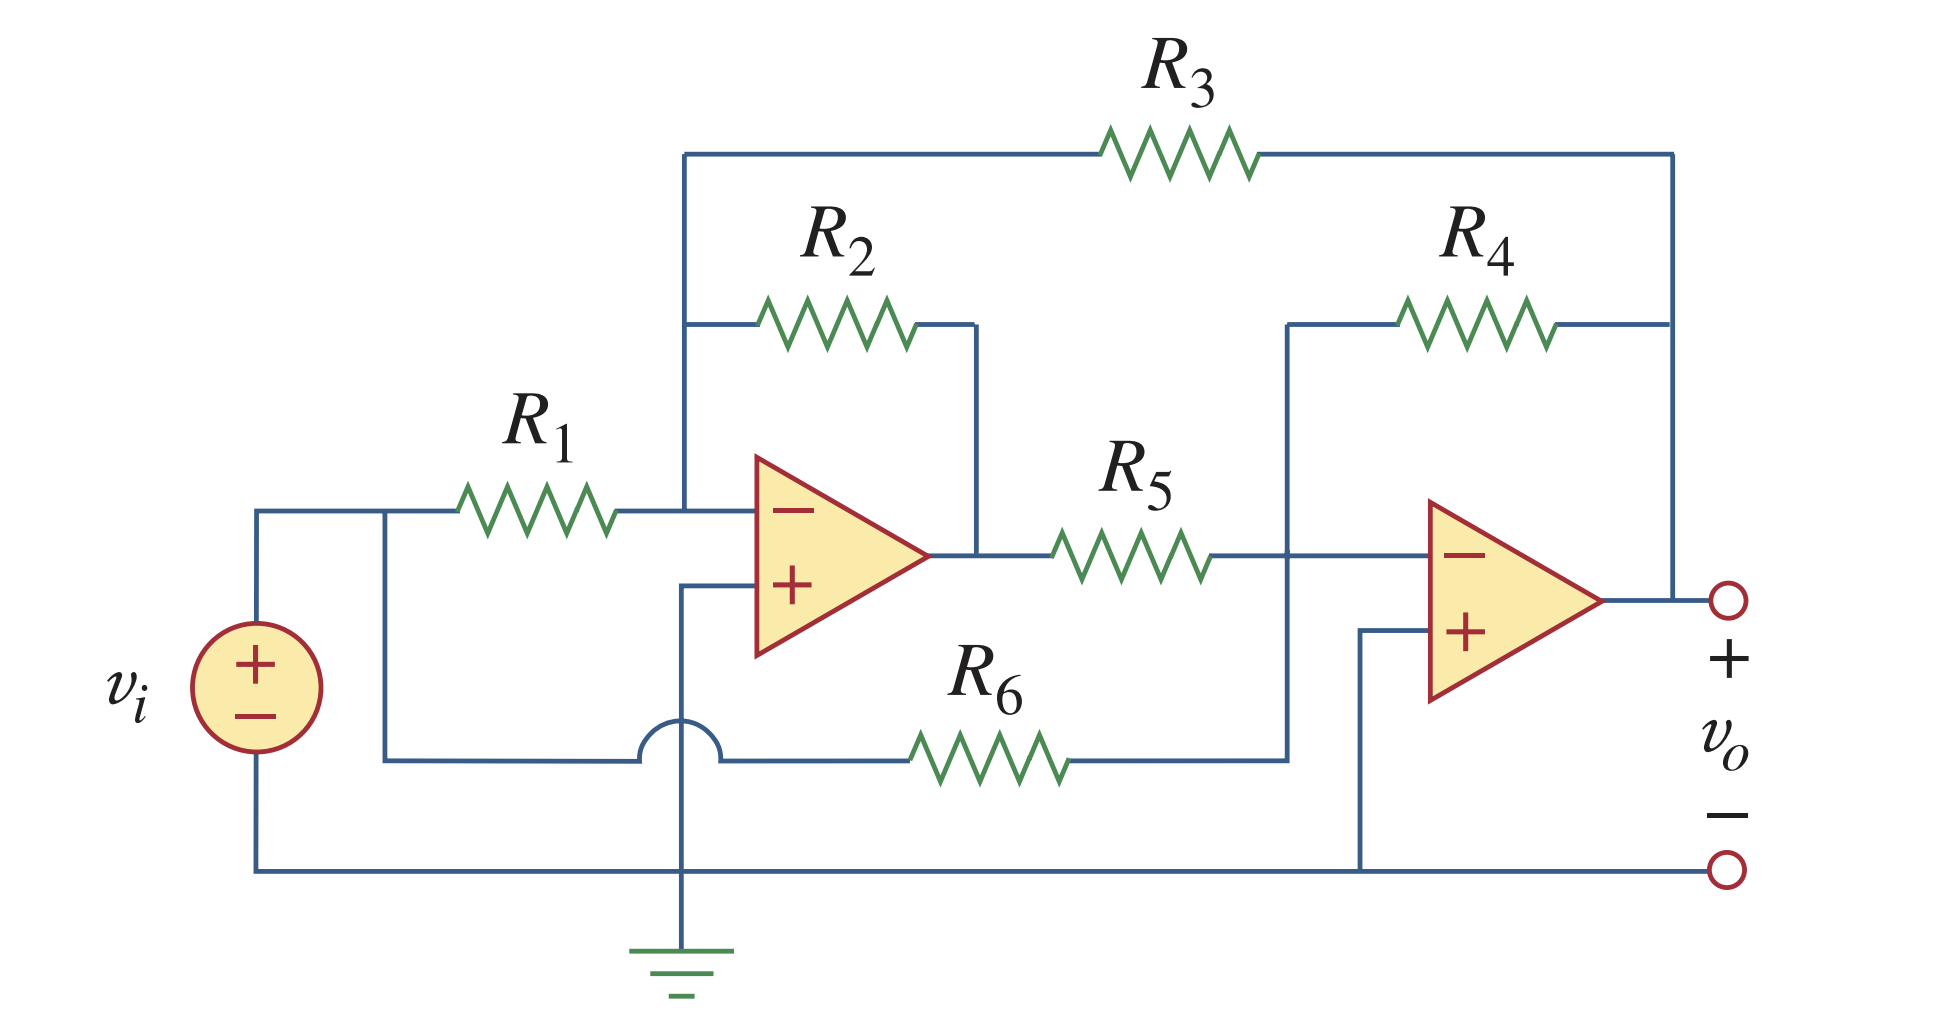
\includegraphics[width=0.8\textwidth]{img_opamp/exercise2.png}
\end{figure}
    
\end{frame}

%%%%%%%%%%%%%%%%%%%%%%%%%%%%%
\begin{frame}{Exercise}
\begin{figure}[H]
    \centering
    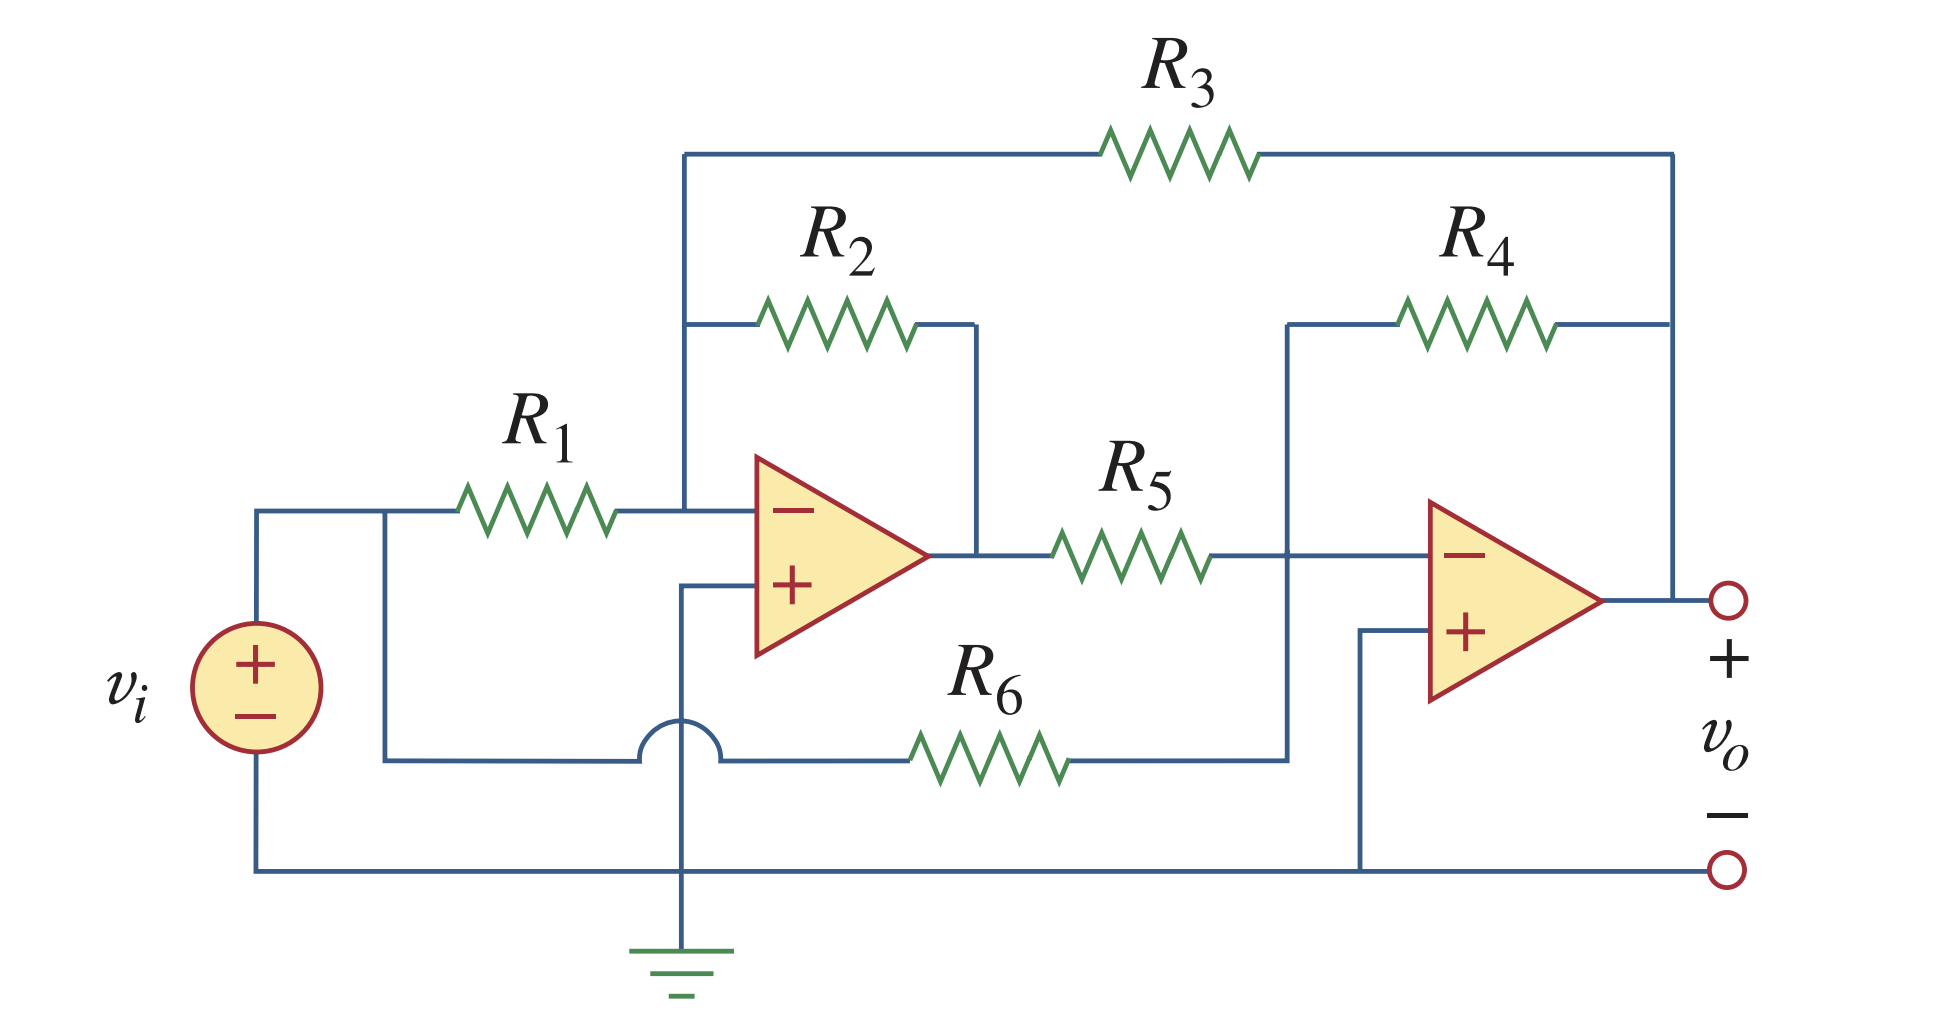
\includegraphics[width=0.65\textwidth]{img_opamp/exercise2.png}
\end{figure}

Answer: $v_o/v_i = \frac{R_2R_4/R_1R_5-R_4R_6}{1-R_2R_4/R_3R_5}$

(Reminder: don't list KCL on the output node)
    
\end{frame}

%%%%%%%%%%%%%%%%%%%%%%%%%%%%%%%%%%%%%%%%%%%%%%%%%%%



\begin{frame}
\frametitle{References}
\begin{enumerate}
\item 2023 Summer VE215 slides, Rui Yang
\item Fundamentals of Electric Circuits, 5th e, Sadiku, Matthew
\item 2022 Fall RC3, Yifei Cai
\end{enumerate}
\end{frame}


\begin{frame}
\Huge{\centerline{Thank you!}}
\end{frame}


\end{document}
